\documentclass{article}
\usepackage[utf8]{inputenc}
\usepackage[spanish]{babel}
\usepackage{graphicx}
\usepackage{verbatim}
\usepackage{moreverb}
\usepackage{amsmath}
\usepackage{amsfonts}
\usepackage{amssymb}
\usepackage{fancybox}
\usepackage{float}
\usepackage{fancyvrb}
\usepackage{color}
\usepackage{url}
\usepackage{multicol}
\usepackage[a4paper, hmargin=2cm, vmargin=2.5cm]{geometry}

%Nuevo comando: Inserta una línea recta.
\newcommand{\HRule}{\rule{\linewidth}{0.5mm}}

\begin{document}

%%%%%%%%%%%%%%%%%%%%%%%%%%%%%%%%% PORTADA %%%%%%%%%%%%%%%%%%%%%%%%%%%%%%%%%%%%%%

\begin{center}

{ \huge \bfseries Un sistema de comunicaciones}\\[0.4cm]

\large Julián Gutiérrez (51141) |
\large Pablo Pauli (51185) |
\large Ivan Itzcovich (53891) |
\large Gustavo Del Giudice (51289)\\[0.3cm] 

\end{center}

%%%%%%%%%%%%%%%%%%%%%%%%%%%%%%%%%%%%%%%%%%%%%%%%%%%%%%%%%%%%%%%%%%%%%%%%%%%%%%%%

% Seteo marcos para lo que esté en el entorno verbatim
\fvset{frame=single}

\begin{abstract}
\par Este trabajo practico  consiste en la estimación de un canal mediante cuadrados mínimos
\end{abstract}

\begin{multicols}{2}

\section{Introducción}


\par Un modelo muy simple de un sistema de comunicaciones consiste de un transmisor que envia un dato cada cierto tiempo.Los datos son modificados por el canal, es decir, por el medio donde son transmitidos.Esta modificacion se genera por la respuesta al impulso del
canal. Además de ser modificados por el canal, los datos son afectados por ruido blanco Gaussiano aditivo. Teniendo en cuenta estas modificaciones, el receptor obtiene una respuesta.\\
\par Lo que nos interesa es, usando la respuesta que obtiene el receptor, conseguir la señal que se envio al inicio de la comunicacion. El problema es que las modificaciones al canal y la longitud de la respuesta al impulso no suelen ser conocidas, por lo tanto deberemos estimarlos. 
Si la longitud es conocida, es posible estimar el canal utilizando cuadrados minimos. Para esto, hay que enviar una señal conocida por el receptor. A esto se lo denomida secuencia de entrenamiento.Luego, se estima el canal planteando otro problema de cuadrados minimos. 



\section{Desarrollo}
\subsection{Subseccion}
\label{sec1}

%\par La Transformada de Fourier puede ser generalizada a varias dimensiones. En nuestro caso, una imagen puede interpretarse como una señal de dos dimensiones, por tanto utilizaremos una generaliación bidimensional de la Transformada de Fourier sobre variables discretas (Ecuación \ref{transform}). Análogamente, para el proceso de anti-transformación utilizamos una generalización bidimensional de la anti-transformada sobre variables discretas (Ecuación \ref{antitransform}). Las funciones  \ref{ftbi} y \ref{ftbiInv} del anexo muestran una simple implementación de las ecuaciones anteriores respectivamente. Sin embargo utilizando diferentes propiedades es posible realizar optimizaciones a las mismas para lograr una mayor eficiencia de cómputo. Es por esto que a fines prácticos utilizamos las funciones \verb+fft2+ y \verb+ifft2+ de \textit{Octave} que calculan la Transformada Rápida de Fourier y la Antitransformada Rápida de Fourier respectivamente.

%\begin{equation}
%\label{transform}
%X_{l,k} = \sum_{n=0}^{N-1}\sum_{m=0}^{N-1} x_{n,m} e^{-i\frac{2\pi}{N}(nl + mk)}
%\end{equation}

%\begin{equation}
%\label{antitransform}
%x_{n,m} = \frac{1}{N^2} \sum_{l=0}^{N-1}\sum_{k=0}^{N-1} X_{l,k} e^{+i\frac{2\pi}{N}(nl + mk)}
%\end{equation}

%\subsection{Imágenes en amplitud y fase}
%\label{sec2}


%\par A modo de ejemplo tomamos una imagen arbitraria, en una escala de 256 grises, llamada \verb+saturno+ (\ref{saturno}). A la misma le aplicamos la Transformada de Fourier en dos dimensiones y remapeando el resultado al intervalo entero $[0,255]$ obtuvimos su representación en fase (\ref{saturnoPhase}), al mismo tiempo aplicando módulo al resultado resultó su representación en amplitud (\ref{saturnoAmplitude}). Para comprobar el proceso podríamos aplicar la Antitransformada de Fourier para obtener nuevamente la imagen original.

\begin{figure}[H]
\centering
\includegraphics[scale=0.2]{../img/lena512.png}
\caption{Imagen 512}
\label{Imagen 512}
\end{figure}

\begin{figure}[H]
\centering
\includegraphics[scale=0.2]{.../mg/lena512.png}
\caption{Imagen 128}
\label{Imagen 128}
\end{figure}

\begin{figure}[H]
\centering
\includegraphics[scale=0.2]{../img/lena512.png}
\caption{Imagen 32}
\label{Imagen 32}
\end{figure}

\par 

\subsection{Subseccion}
\label{sec3}
%\par Un filtro es una función que opera contra la representación en fase de una señal, existiendo así diferentes tipos de filtros según su comportamiento. Los filtros pasa bajos son aquellos que eliminan las altas frecuencias y, en el campo de las imágenes, permiten suavizar una imagen, eliminar ruido y detalles pequeños de poco interés ya que sólo afecta a zonas con muchos cambios. Por otro lado, los filtros pasa alto, quienes eliminan las bajas frecuencias, intensifican detalles, bordes y cambios de alta frecuencia y atenúan las zonas de tonos uniformes.

%\par Para aplicar un filtro a una imagen es necesario representarlo inicialmente como una matriz, como así también la imagen con la sobre la que se operará. Luego debemos aplicar la Transformada de Fourier a esta imagen, multiplicar elemento a elemento el resultado contra el filtro y, finalmente aplicar la Antitransformada de Fourier al resultado para recuperar la imagen filtrada. Es decir, los filtros se aplican en la frecuencia. Si $x$ es la matriz que contiene a la imagen, $X$ será su transformada y $xfil$ será la imagen con el filtro aplicado. Se denomina $H$ al filtro y $F$ a la Transformada Discreta de Fourier Bidimensional.

%\begin{eqnarray*}
%    X &=& F(x)\\
%    xfil &=& F^{-1}(H * X)
%\end{eqnarray*}

%\par Para ejemplificar la utilización de los filtros implementamos tres diferentes y su definición se presenta a continaución:

%\begin{itemize}
%    \item \begin{equation} H_{k,l} = \left\{ \begin{array}{lr}
%                                0 & \textnormal{ si } 0 \le k \le 400, 190 \le l \le 210\\
%                                0 & \textnormal{ si } 190 \le k \le 210, 0 \le l \le 400\\
%                                1 & \textnormal { en otro caso }
%                               \end{array}
%              \right. 
%          \end{equation}\\
%    \item Filtro Gaussiano \begin{equation} H_{k,l} = e^{ -0.01 (k^2 + l^2)} \end{equation}\\
%    \item El damero \begin{equation} H_{k,l} = \left\{ \begin{array}{lr}
%                                0 & \textnormal{ si } l + k \textnormal{ es par }\\
%                                1 & \textnormal{ si } l + k \textnormal{ es par }
%                               \end{array}
%              \right. 
%          \end{equation}
%\end{itemize}

\section{Resultados y conclusiones}
\label{sec4}

\begin{figure}[H]
\centering
\includegraphics[scale=0.2]{../img/lena512.png}
\caption{Imagen 512}
\label{Imagen 512}
\end{figure}

\begin{figure}[H]
\centering
\includegraphics[scale=0.2]{../img/lena512.png}
\caption{Imagen 128}
\label{Imagen 128}
\end{figure}

\begin{figure}[H]
\centering
\includegraphics[scale=0.2]{../img/lena512.png}
\caption{Imagen 32}
\label{Imagen 32}
\end{figure}


\par Sarasa de las concluciones \textit{Octave}.\\

\end{multicols}

\section{Bibliografía} 

\begin{itemize}
  \item Fierens, Pablo. \textit{Guía 1}, Métodos Numéricos Avanzados. ITBA, 1er Cuatrimestre 2014

\end{itemize}

\clearpage

\section{Anexo}
\par Aquí se pueden ver las funciones de \textit{GNU Octave} utilizadas para este análisis.\\

\par El \textit{script} \verb+initializeCannal.m+ inicializa las variables del canal.

\begin{ttfamily}
\begin{center}
\fbox{\parbox{6in}{\textbf{initializeCannal.m} \\
\verbatiminput{../src/initializeCannal.m}
}}
\end{center}
\end{ttfamily}

\par El \textit{script} \verb+simulation.m+ implementa la simulacion del sistema de comunicacion .

\begin{ttfamily}
\begin{center}
\fbox{\parbox{6in}{\textbf{simulation.m} \\
\verbatiminput{../src/simulation.m}
}}
\end{center}
\end{ttfamily}

\par El \textit{script} \verb+train.m+ implementa la secuencia de entrenamiento.

\begin{ttfamily}
\begin{center}
\fbox{\parbox{6in}{\textbf{train.m} \\
\verbatiminput{../src/train.m}
}}
\end{center}
\end{ttfamily}

\par El \textit{script} \verb+transmit.m+ simula la transmicion por el canal.

\begin{ttfamily}
\begin{center}
\fbox{\parbox{6in}{\textbf{transmit.m} \\
\verbatiminput{../src/transmit.m}
}}
\end{center}
\end{ttfamily}

\par El \textit{script} \verb+cholesky.m+ obtiene la descomposición de Cholesky de una matriz simétrica.

\begin{ttfamily}
\begin{center}
\fbox{\parbox{6in}{\textbf{cholesky.m} \\
\verbatiminput{../src/cholesky.m}
}}
\end{center}
\end{ttfamily}

\par El \textit{script} \verb+minimumSquares.m+ resuelve los cuadrados mínimos por Cholesky.

\begin{ttfamily}
\begin{center}
\fbox{\parbox{6in}{\textbf{minimumSquares.m} \\
\verbatiminput{../src/minimumSquares.m}
}}
\end{center}
\end{ttfamily}

\par El \textit{script} \verb+backSustitution.m+ hace la sustitucion hacia atras.

\begin{ttfamily}
\begin{center}
\fbox{\parbox{6in}{\textbf{backSustitution.m} \\
\verbatiminput{../src/backSustitution.m}
}}
\end{center}
\end{ttfamily}


\par El \textit{script} \verb+saveImages.m+ guarda las imagenes.

\begin{ttfamily}
\begin{center}
\fbox{\parbox{6in}{\textbf{saveImages.m} \\
\verbatiminput{../src/saveImages.m}
}}
\end{center}
\end{ttfamily}

\par El \textit{script} \verb+calculatehError.m+ calcula el error de h.

\begin{ttfamily}
\begin{center}
\fbox{\parbox{6in}{\textbf{calculatehError.m} \\
\verbatiminput{../src/calculatehError.m}
}}
\end{center}
\end{ttfamily}


\par El \textit{script} \verb+estimateh.m+ estima el valor de h.

\begin{ttfamily}
\begin{center}
\fbox{\parbox{6in}{\textbf{estimateh.m} \\
\verbatiminput{../src/estimateh.m}
}}
\end{center}
\end{ttfamily}

\end{document}
